%Idet ASP.NET Core MVC benyttes i Weplanner projektet, medfører det en overordnet meget lav kobling. Dette medfører at integrationstests ikke er nødvendige på tværs af Controllers da de ikke har noget med hinanden at gøre. Dog kan det være en god idé at lave UnitTests for controller, samt en integrationstest mellem DAL og en database. Unit-Testing af en controller kan sikre at flowet af koden i de forskellige Actions forløber som forventet, og kan opdage fejl der opstår ved modificering af koden. 
%Unit-Test af DAL, giver ikke rigtigt mening, da logikken i denne er forholdsvist simpel, hvorved udbyttet af disse UnitTests ikke vil være særligt givende. Dog kan det være en god idé at lave en integrationstest mellem DAL og en database. Disse tests kan køres automatisk, fx. på en Jenkins server\cite{Jenkins}, hver gang der bliver pushet til projektets repository. Fejl kan da automatisk detekteres og udviklere notificeres herom. Hvis testene er skrevet ordentligt bør det være nemt at finde fejlen og rette denne til. Dog er det tidskrævende at skrive Tests, og efter at have skrevet nogle tests, vurderes udbyttet af disse, til ikke at være tiden værd, idet det opleves at eventuelle fejl i projektet er nemme at finde, grundet den lave kobling. 

%Der laver derfor kun Unit-Test for én controller, samt integrations test med ét repository. Booking controlleren, samt Booking-repository vælges fordi Booking-widgetten har været beskrevet udførligt i rapporten. NUnit \cite{NUnit}, som anvendes i faget SWT, anvendes som Unit-Testing framework, og NSubstitute\cite{NSubstitute} anvendes til at Mocke BookingRepository til Unit-Test af BookingControlleren. 

\section{Unit Test}
Idet ASP.NET Core MVC benyttes i Weplanner projektet, medfører det en overordnet meget lav kobling. Dette medfører at integrationstests ikke er nødvendige på tværs af Controllers da de ikke har noget med hinanden at gøre. Dog kan det være en god idé at lave UnitTests for controller. Unit-Testing af en controller kan sikre at flowet af koden i de forskellige Actions forløber som forventet, og kan opdage fejl der opstår ved modificering af koden. I dette afsnit gennemgås det hvordan der er lavet unit test for BookingController'en. 

De forskellige funktioner i BookingController'en testes for om de returnerer det forventede output på baggrund af et givent input. Der laves både Black-Box tests og White-box tests af controlleren. Et eksempel på en Black-box test kunne være at undersøge om statuskoden på returværdien for funktionen, stemmer overens med den forventede. Fx. hvis en reservation med et bestemt ID ikke findes, bør der returneres noget med en statuskode på 404(NotFound), hvis en bruger prøver at redigere en reservation med dette ID. Et eksempel på sådan en test kan ses herunder på figur \ref{fig:Test_BookingDeleteReservation}.   

\begin{figure}[H]
  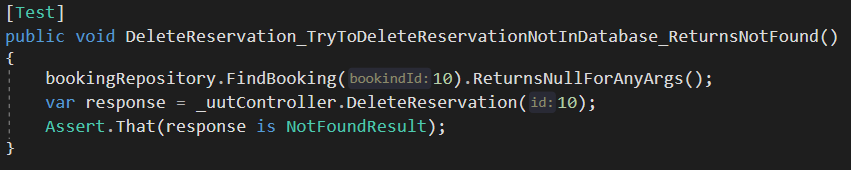
\includegraphics[width=0.8\linewidth]{01_Billeder/11_Test/Booking_TestDeleteReservation.png}
  \centering
  \caption{Eksempel på Black-Box test af BookingController, hvor der forsøges at slette en reservation der ikke eksisterer}
  \label{fig:Test_BookingDeleteReservation}
\end{figure}

White-box tests af BookingControlleren kan fx. være med til at sikre, at der ikke kan oprettes flere booking-systemer for en gruppe. Et eksempel på sådan en test kan ses på figur \ref{fig:Test_BookingExists}.


\begin{figure}[H]
  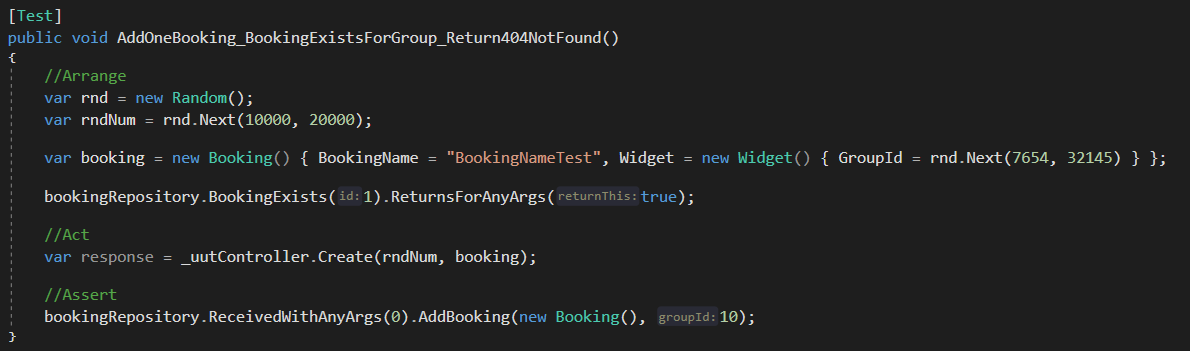
\includegraphics[width=\linewidth]{01_Billeder/11_Test/Booking_TestBookingExists.png}
  \centering
  \caption{Eksempel på White-box test af BookingController, hvor der forsøges at oprette et booking-system i en gruppe der allerede indeholder ét booking-system.}
  \label{fig:Test_BookingExists}
\end{figure}

Flere tests af Booking-controlleren kan findes i source koden.
\store{ref til bilag.}

\section{Integrationstest}
Der hvor det giver mening at lave integrationstest er mellem DAL og en database. I dette afsnit laves der integrationstest mellem DAL for BookingController'en og databasen. Denne integrationstest laves for at sikre at de forventede data rent faktisk gemmes korrekt i databasen. 
\\ \\
I stedet for den rigtige database, anvendes i stedet en In-memory SQLite database, som simmulerer den rigtige database. In-memory databasen kan kontrolleres bedere, og testenes resultat er da ikke afhængig af forbindelse til en ekstern database. Samtidigt kunne andre brugere potentielt gå ind og slette/redigere data i den eksterne database som kan ødelægge disse tests. 
\\ \\
Hver tests består essentielt set af to ting. Indledningsvist kaldes en eller flere funktioner hvor der indsættes/slettes eller opdateres data i databasen. Herefter undersøges der om det foreventede data eksisterer i databasen. Indledningsvist testes om funktioner der indsætter data, virker. Disse funktioner kan da bruges i de efterfølgende tests. En anden ting der testes for, er om fx. når en ressource(BookingItem) slettes, at dens tilhørende reservationer og dens tilhørende events også slettes. Et eksempel på en sådan tests kan ses på figur \ref{fig:Test_BookingDAL}.   

\begin{figure}[H]
  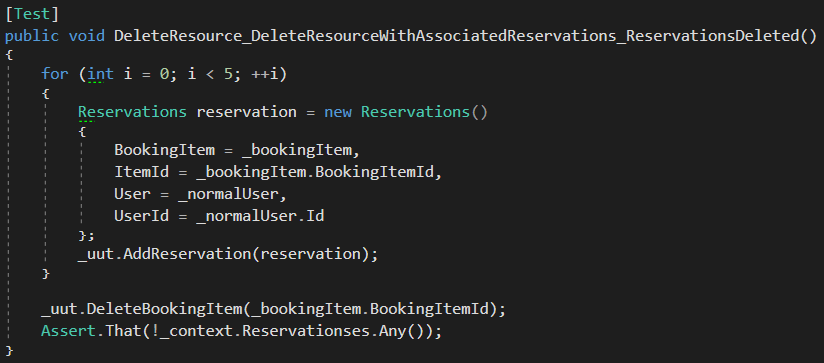
\includegraphics[width=\linewidth]{01_Billeder/11_Test/Booking_TestDAL.png}
  \centering
  \caption{Eksempel på en integrationstest af DAL med In-memory database. Der testes for om reservationer tilhørende en ressource også slettes, hvis ressource slettes}
  \label{fig:Test_BookingDAL}
\end{figure}

\section{Fremtidige overvejelser}

Under udviklingen af disse tests erfares det at det er meget tidskrævende, samt at udbyttet ikke er særligt stort. Der overvejes derfor andre mindre tidskrævende muligheder, som kan hjælpe med at finde fejl. En mulighed kunne være at implementere et logging system som logger alle fejl der opstår igennem applikationen. Hertil findes der mange online værktøjer som kan bruges til dette, fx Stackify \cite{Stackify}. Dette kan dog ikke nødvendigvis finde eventuelle 'huller' i vores database. En måde hvorpå dette kan kunne undersøges, var at implementere en form for feedback system, hvor brugere kan rapportere bugs som de finder. Disse kan da undersøges og fixes af udviklerne. Eventuelt, kan man også skrive lave en integrationstest af hvert DAL med en tilhørende database. 